\documentclass{article}
\usepackage{graphicx}
\graphicspath{ {./../pix/} }
\usepackage{wrapfig}
\usepackage{xcolor}
\definecolor{light-gray}{gray}{0.95}
\newcommand{\code}[1]{\colorbox{light-gray}{\texttt{#1}}}
\usepackage[utf8]{inputenc}
\usepackage[english]{babel}
\usepackage[]{amsthm}
\usepackage[]{amssymb}

\title{1729 Project}
\author{Ian Turner}

\begin{document}
\maketitle
\section*{Quantum Computing For The Very Curious}
\textit{I will use this section document to study this essay on quantum
computing. I am not quite sure how to take notes on this yet, but I will
figure something out.}

\subsection*{Measuring a quibit}
The key takeaway from this section is that the values of $\alpha$ and $\beta$ can never
be determined; in other words, they are hidden information.\\
\textbf{Example}

\begin{figure}[h]
    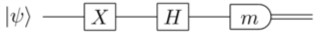
\includegraphics[width=6cm]{1.jpg}
    \centering
\end{figure}

it's a single-quibit quantum circuit, with input the state $|$$\psi$$\rangle$.
A NOT gate is applied, followed by a Hadmard gate. The circuit finishes with a
measurement in the computational basis, denoted by the slightly enongated semi-
circle. The \textit{m} is a classical bit denoting the measurement result 0, or
1. We use the double wire to indicate the classical bit \textit{m} going off
and being used to do something else.

\subsection*{General Single-Qubit Gates}
Let's look at the most general single-qubit gate. Recall the matrix
representations of the NOT and Hadamard gates:

\begin{figure}[h]
    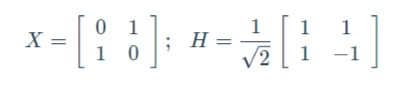
\includegraphics[width=6cm]{2.jpg}
    \centering
\end{figure}

If the input to these gates is the quantum state $|$$\psi$$\rangle$, then
the output is $|$$X$$\rangle$ and  $|$$H$$\rangle$ respectively. In general,
a single quibit gate can be represented as a 2x2 unitary matrix, $U$. What does
it mean for a matrix $U$ to be unitary? It simply means that $U^\dagger U$ :=
$(U^T)^*$. The $\dagger$ is also sometimes called the \textit{dagger operation}
, or \textit{Hermitian conjugation}, or just the \textit{conjugation} operation.

\textbf{Example}
Let's start by checking the unitarity of the Hadamard gate, We start by
computing the adjoint of H:

\begin{figure}[h]
    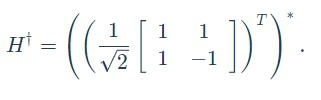
\includegraphics[width=6cm]{3.jpg}
    \centering
\end{figure}

Note that taking the transpose doesn't change the matrix, since it is already
symmetric. And taking the complex conjgate doesn't change anything, since
all the entries are real. So we have $H^\dagger = H$, and thus $H^\dagger H = HH$.
so $H$ is, indeed, unitary.

\subsection*{What Does it Mean for a Matrix to be Unitary?}
Can we get an intuition for what it means for a matrix to be unitary? It turns
out that unitary matrices \textit{preserve the length of their inputs}. In
other words, if we take any vector $|\psi\rangle$ and compute the length $||U|\psi\rangle||$
it's always equal to the length $|||\psi\rangle||$ of the original vector.

\subsection{The Controlled-NOT Gate}

\begin{figure}[h]
    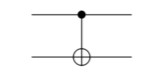
\includegraphics[width=6cm]{4.jpg}
    \centering
\end{figure}

The wire with the small, filled dot on it is called the \textit{control} qubit,
for reasons which will become clear in a moment. An the wire with the larger,
unfilled circle on it is called the \textit{target} qubit.

The CNOT gate gives us 4 basic computational states:

\begin{figure}[h]
    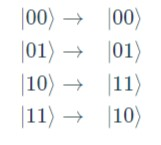
\includegraphics[width=3cm]{5.jpg}
    \centering
\end{figure}

If you're familiar with classical programming languages, then you can think of
the CNOT as a very simple kind of \code{if-then} statement: \code{if} the
control qubit is set, \code{then} NOT the target qubit. But while simple, it
can be used as a building block to build up other, more complex kinds of
conditional behavior.\\
There's a way of summing up all four of the equations above in a single
equation. Suppose $x$ and $y$ are classical bits, i.e., 0 or 1. Then we can
rewrite the equations above in a single equation as: $|x,y\rangle\rightarrow |x,y\oplus x\rangle$.
Note the commas inserted to make this easier to read -- this is pretty common
in working with multi-qubit states. \\
The above equation makes clear that the CNOT leaves the control qubit $x$ alone,
but flips the target qubit $y$ if $x$ is set to 1. Note that $\oplus$ is addition
modulo 2, where $1 \oplus 1 = 0$, as we would expect from the fact that CNOT
takes $|11\rangle$ to $|10\rangle$.\\
That's all there is to the CNOT. It's really a very simple idea and quantum
gate. Note that it of course acts linearly on superpositions of computational
basis states, as we expect for a quantum gate.

\Section{Part III: Universal Quantum Computing}





































\end{document}
